\def\difficulty{2}
\sujet{Voronoï Diagrams and Delaunay Triangulation}
\index{Computational Geometry!Voronoi Diagram}
\index{Computational Geometry!Delaunay Triangulation}
\index{Computational Geometry!Minimum Spanning Tree}

\begin{note}
This tutorial aims to spatially characterize a spatial point pattern by using some 
tools of computational geometry: the Voronoi diagram, 
the Delaunay triangulation and the Minimum Spanning Tree (MST), illustrated in Fig.\ref{fig:point_processes_voronoi:enonce:geometry}.

For biomedical issues, this point pattern analysis can help the biologists 
to classify different populations of cells.
\end{note}

\begin{figure}[htbp]
 \centering\caption{Random point pattern and some geometrical structures used to characterize it.}%
 \subfloat[Initial points]{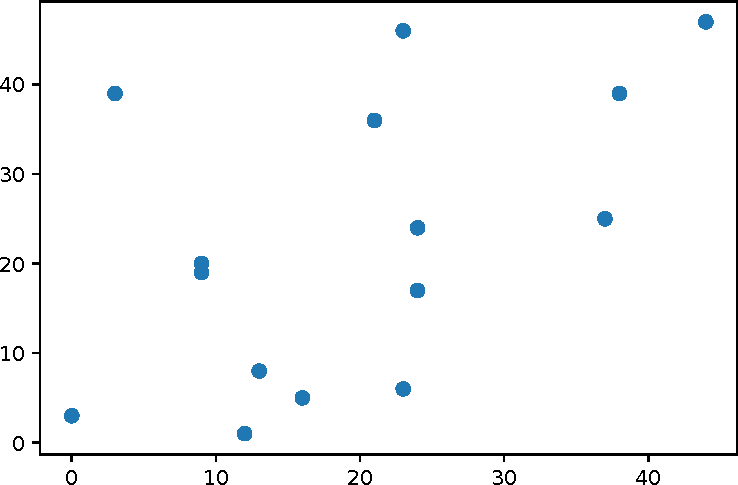
\includegraphics[width=.45\linewidth]{points-crop.pdf}}\hfill
 \subfloat[Voronoi diagram]{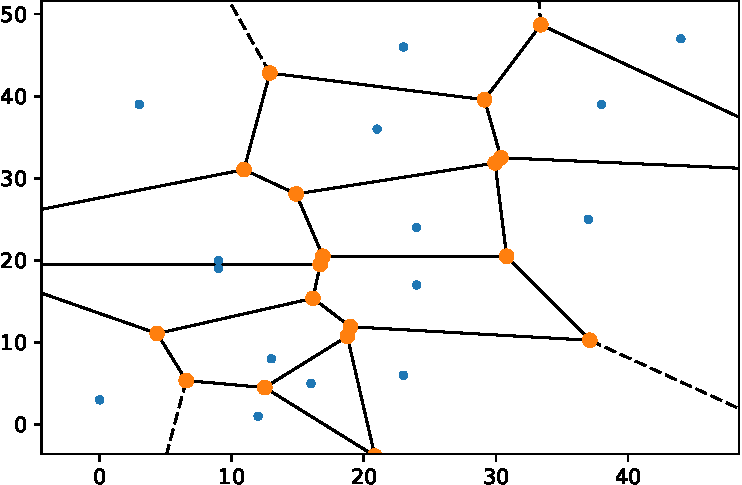
\includegraphics[width=.45\linewidth]{voronoi-crop.pdf}}
 
 \subfloat[Delaunay triangulation]{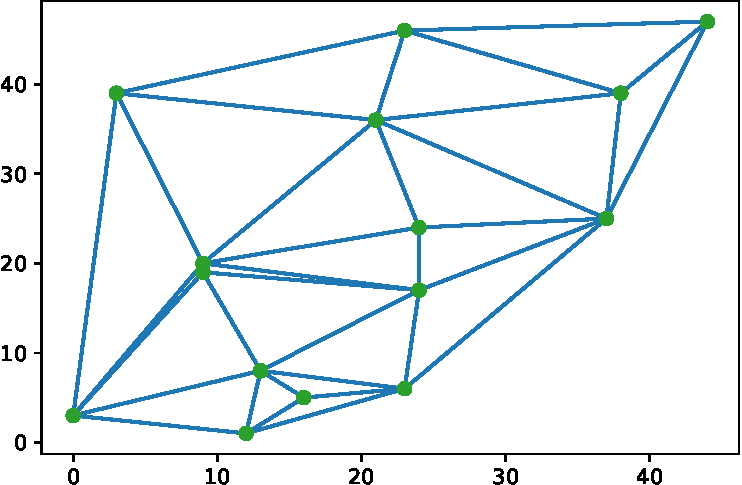
\includegraphics[width=.45\linewidth]{delaunay-crop.pdf}}\hfill
 \subfloat[Minimum spanning tree of the Delaunay triangulation]{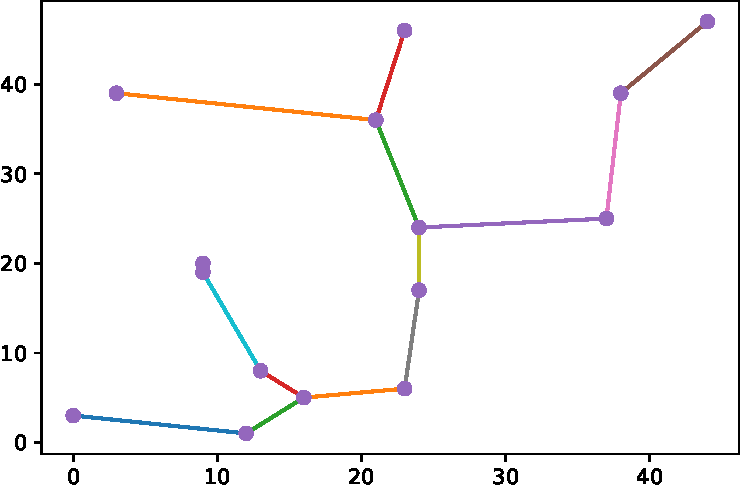
\includegraphics[width=.45\linewidth]{mst-crop.pdf}}%
 \label{fig:point_processes_voronoi:enonce:geometry}%
\end{figure}


\section{Voronoi and Delaunay}%, Delaunay, Minimum Spanning Tree}
A voronoi diagram, in 2D, is defined as a partition of the plane into cells $R_k$ according to a distance function $d$ and a set of seeds 
(germs) $P_k$. 
$$R_k = \{x \in X \mid d(x, P_k) \leq d(x, P_j)\; \text{for all}\; j \neq k\}$$
The Delaunay graph is the dual graph that links the germs of the neighborhing Voronoi cells.

\subsection{Random tesselation}
Follow these instructions to generate a random tesselation:
\begin{qbox}
\begin{enumerate}
	\item Generate a random point process.
	\item Determine the Delaunay triangulation.
	\item Determine the Voronoi diagram.
	%\item Determine the minimum spanning tree with the \matlabregistered{} function 
	%\minline{minspantree} (introduced in Matlab 2015b) or \minline{graphminspantree}. It uses Kruskal's algorithm.
\end{enumerate}
\end{qbox}

\begin{mcomment}
\begin{mremark} Use the \matlabregistered{} functions \minline{delaunayTriangulation} and \minline{voronoiDiagram}.
\end{mremark}
\end{mcomment}

\begin{pcomment}
\begin{premark}
 Use the python functions \pinline{Delaunay} and \pinline{Voronoi} from \pinline{scipy.spatial}.
\end{premark}
\end{pcomment}


\subsection{Characterization of the Voronoi diagram}
This basic approach characterizes the set of the cells. With the help of the Voronoi diagram, it is possible to make the two following measurements,
Area Disorder (AD) and Round Factor Homogeneity (RFH), defined by:
	\begin{eqnarray}
	AD&=&1-\frac{1}{1+\displaystyle\frac{\sigma(A)}{\mu(A)}}\\
	RFH&=&1-\frac{\sigma(RF)}{\mu(RF)}
	\end{eqnarray}
	where $A$ and $RF$ are calculated on the regions $R_k$ of the Voronoi diagram.  $\mu$ and $\sigma$ are the mean and standard 
deviation of the areas of the Voronoi cells. The circularity (RF) of a polygon can be defined as the ratio between its area and the area of the disk of an equivalent perimeter.


\begin{qbox}
 \begin{itemize}
  \item Code these measurements with the following prototypes:
  \begin{matlab}
function ad = AD(V, R)
% computes AD (area disorder) parameters
% V: Vertices of the Voronoi diagram
% R: Regions of the Voronoi diagram
  \end{matlab}
  
  \begin{python}
def AD(vor):
# takes a voronoi diagram to compute area disorder
  \end{python}
  
  In order to evaluate the area of each Voronoi cell, transform each cell to a polygon. 

\item Represent the couple $(ad,rfh)$ in a graph, which gives a characterization of the Voronoi diagram.
 \end{itemize}
\end{qbox}

\begin{mcomment}
\begin{mremark}
See \minline{polyarea} for evaluating the area of a polygon.
\end{mremark}
\end{mcomment}

\begin{pcomment}
\begin{premark}
See \pinline{shapely.geometry.Polygon} for evaluating the area of a polygon.
\end{premark}
\end{pcomment}


\subsection{Characterization of the Delaunay graph}
If $L$ denotes the set of the edge lengths of the Delaunay triangulation, the mean and the standard deviation of $L$ 
can also give informations on the graph.
\begin{qbox}
 \begin{itemize}
  \item Compute and display in a graph the point of coordinates $(\mu(L), \sigma(L))$, with $\mu$ representing the mean 
  and $\sigma$ the standard deviation.
 \end{itemize}

\end{qbox}

\section{Minimum spanning tree}
Definition from Wikipedia: a minimum spanning tree (MST) or minimum weight spanning tree is a subset of the edges of a connected, edge-weighted undirected graph that connects all the vertices together, without any cycles and with the minimum possible total edge weight. 
That is, it is a spanning tree whose sum of edge weights is as small as possible.

One of the methods to compute the MST is the Kruskal algorithm. 

\begin{mcomment}
\begin{mremark}
It is implemented in Matlab via the function 
\minline{minspantree} (introduced in \matlabregistered{} 2015b) or \minline{graphminspantree}.
\end{mremark}
\end{mcomment}

\begin{qbox}
 \begin{itemize}
 \item Compute the MST.
  \item  Compute $(\mu(L^*),\sigma(L^*))$ where $L^*$ denotes the set of the edge lengths of the 
MST.
 \end{itemize}
\end{qbox}


\section{Characterization of various point patterns}
\begin{qbox}
\begin{enumerate}
	\item Generate $n$ condition Poisson point processes of $100$ points each. For each realization, calculate the parameters $(AD,RFH)$, 
$(\mu(L),\sigma(L))$ and $(\mu(L^*),\sigma(L^*))$. Display these $n$ points in a 2D diagram in order to analyze the robustness of the 
quantification.
	\item Generate 3 different point processes with regular, uniform and Gaussian dispersion. Display the different diagrams. Which one 
is the most discriminant?
\end{enumerate}
\end{qbox}
